\documentclass{beamer}
\usepackage[utf8]{inputenc}

\usepackage[spanish,activeacute,es-tabla]{babel}
\usepackage[utf8]{inputenc} % mac utf8
\usepackage{beamerthemesplit}
\usepackage{booktabs}
\usepackage{siunitx}
\usepackage{listings}
\usepackage{xcolor}
\usepackage{graphicx}
\DeclareGraphicsExtensions{.png,.pdf,.jpg}


\usefonttheme{professionalfonts} % fuentes de LaTeX 
\usetheme{Boadilla}	% tema escogido en este ejemplo 


\setbeamertemplate{caption}[numbered]

\newtheorem{Teorema}{Teorema} 
\newtheorem{Definicion}{Definici\’on} 
\newtheorem{Prueba}{Prueba}

\theoremstyle{plain}

\newtheorem{teorema} [Teorema] {Teorema}
\newtheorem{definicion} [Definicion]{Definición} 
\newtheorem{lema} [theorem] {Lema}


\theoremstyle{example}
\newtheorem{Ejercicio}{Ejercicio} 
\newtheorem{ejercicio} [Ejercicio]{Ejercicio} 

\theoremstyle{example}
\newtheorem{Ejemplo}{Ejemplo} 
\newtheorem{ejemplo} [Ejemplo] {Ejemplo}

\setbeamertemplate{theorems}[numbered] 

% 3) Colores por defecto del style 'example' (fallback)
\setbeamercolor{block title example}{bg=green!40!black, fg=white}
\setbeamercolor{block body example}{bg=green!10, fg=black}

% 4) Colores por ENTORNO (locales) usando etoolbox
\usepackage{etoolbox}

% -- 'Ejemplo' en naranja
\AtBeginEnvironment{ejemplo}{%
  \setbeamercolor{block title example}{bg=orange!60!black, fg=white}%
  \setbeamercolor{block body example}{bg=orange!10, fg=black}%
}
% -- 'Ejercicio' en violeta
\AtBeginEnvironment{ejercicio}{%
  \setbeamercolor{block title example}{bg=violet!60!black, fg=white}%
  \setbeamercolor{block body example}{bg=violet!10, fg=black}%
}


\definecolor{codebg}{RGB}{248,248,248}
\lstset{
  basicstyle=\ttfamily\footnotesize,
  backgroundcolor=\color{codebg},
  frame=single,
  breaklines=true,
  showstringspaces=false,
  columns=fullflexible
}

\title[]{Tema 4. Compresión de Datos}
\author[José A Montenegro (jmmontes@uma.es)]{José A. Montenegro}
\institute{Dpto. Lenguajes y Ciencias de la Computación\\
ETSI Informática. Universidad de Málaga\\
jmmontes@uma.es
%\href{https://twitter.com//monteDocencia}{
%
\includegraphics[height=0.03\textheight]{twitter.jpg}}
}
\date{\today}

%###########################################################################
% FootLine
%###########################################################################

\setbeamertemplate{footline} {%
\leavevmode%
  \hbox{\begin{beamercolorbox}[wd=.5\paperwidth,ht=2.5ex,dp=1.125ex,leftskip=.3cm plus1fill,rightskip=.3cm]{author in head/foot}%
    \usebeamerfont{author in head/foot}\insertshortauthor 
  \end{beamercolorbox}%
  
  \begin{beamercolorbox}[wd=.5\paperwidth,ht=2.5ex,dp=1.125ex,leftskip=.3cm,rightskip=.3cm plus1fil]{title in head/foot}%
    Teoría de la Información y Codificación \hfill    \insertpagenumber /\insertdocumentendpage
  \end{beamercolorbox}}%
  \vskip0pt%
}%

%###########################################################################
% Document
%###########################################################################

\begin{document}

%\setbeamertemplate{headline}[title slide]
%\setbeamertemplate{footline}[title slide]


%###########################################################################
% Tíitulo
%###########################################################################
\begin{frame}

\includegraphics[height=0.15\textheight]{logoUma.jpg} \hspace*{3.5cm}

\includegraphics[height=0.17\textheight]{logoInf.jpg}   \hspace*{3.5cm}

\includegraphics[height=0.17\textheight]{logoLcc.jpg}  

\titlepage


\setbeamertemplate{footline}[body]
\setbeamertemplate{headline}[body]
\end{frame}

%###########################################################################
% Contenidos
%###########################################################################

\section[Resumen]{}
\frame{\tableofcontents}


\section{Codificación en bloques} 

\begin{frame}   \footnotesize
{
\setbeamercolor{block title}{bg=blue!60!black, fg=white}
\setbeamercolor{block body}{bg=blue!10, fg=black}
\begin{block}{Sección 1}
Codificación en bloques
\end{block}
}
\end{frame} 


\begin{frame}     \small

\begin{itemize}
\item Hemos formalizado la codificación como una función $c: S\rightarrow T^{*}$ que reemplaza los símbolos de un alfabeto S por cadenas de símbolos en un Alfabeto $T$. 

\item Aunque inicialmente hemos establecido los elementos de S como \textbf{objetos simples}, tales como letras de un alfabeto natural, no hay necesidad lógica para esta restricción. 

\item En la práctica, a menudo es útil dividir la cadena de símbolos emitido por una fuente en \textbf{bloques}  y tratar a los bloques creados como símbolos.

\item Por ejemplo, supongamos que una fuente emite una cadena de letras, con las letras x,y o z, por lo que una cadena típica podría ser:

\begin{center}
$yzxxzyxzyxzzyxxzyzxzzyyy \ldots$
\end{center}

\end{itemize}
 

\end{frame}


%%%%%%%%%%%%%%%%%%
\begin{frame}  \small 

\begin{itemize}
\item
En este ejemplo el alfabeto S es el conjunto \{x,y,z\}.  Por otro lado, podemos dividir la cadena en bloques de longitud 2:

\begin{center}
$yz$ $xx$ $zy$ $xz$ $yx$ $zz$ $yx$ $xz$ $yz$ $xz$ $zy$ $yy$ $\ldots$
\end{center}

\item Ahora el alfabeto es el conjunto $S^{2}$ de pares ordenados:

\begin{center}
$S^{2} =\{xx,xy,xz,yx,yy,yz,zx,zy,zz\}.$
\end{center}

\item Anteriormente, hemos considerado el problema de codificar la fuente (S,p) para que la longitud media de palabra L sea tan pequeña como sea posible.

\item Hemos hallado que la entropía $H_b(p)$  es el límite inferior para L, pero este límite es rara vez alcanzado. 

\item Ahora explicaremos como codificar en bloques nos permite acercarnos más fácilmente  al límite inferior. 
\end{itemize}
\end{frame} 


%%%%%%%%%%%%%%%%%%%%%%%%%%%%%%%%
\begin{frame}  \small 

\begin{ejemplo}

Consideremos un escáner que procesa un documento en blanco y negro. Supongamos que emite B (pixel blanco) y N (pixel negro) con probabilidades $p_B = 0.9$ y $p_N = 0.1$. Calcula la entropía de esta distribución, asumiendo que la fuente es sin memoria, encontrando los mejores código binarios para utilizar bloques de tamaño 1, 2 y 3.\\
\end{ejemplo}	

\pause
\footnotesize

\textit{\underline{Solución}}:\\
La entropía es:

\begin{center}
 $H(p) = 0.9 \times log_2(1/0.9) + 0.1  \times log_2(1/0.1) \approx 0.469.$
\end{center}


\begin{itemize}

\item Utilizando \textcolor{red}{bloques de tamaño 1}, la mejor forma para codificar la fuente es $B \mapsto 0, N \mapsto 1$ debido a que otro código debería utilizar una codificación mayor que 1.

\begin{itemize}  \footnotesize
\item
Por tanto, este código tiene una longitud media de palabra $L_1=$ \textcolor{red}{1}, el cual es peor que el límite inferior establecido en la entropía 0.469. 

\item
Un documento que contiene N pixels es codificado como una cadena de N bits, aunque desde el punto de vista teórica, la cantidad de información es equivalente solamente a \textcolor{blue}{0.469N} bits.
\end{itemize}

\item ... continua 

\end{itemize}
\end{frame} 

%%%%%%%%%%%%%%%%%%%%%%%%%%%%%%%%
\begin{frame}  \footnotesize 

\begin{itemize}

\item Consideramos que ocurre cuando dividimos el mensaje en \textcolor{red}{bloques de tamaño 2}. Ahora tenemos una fuente con 4 símbolos, y las probabilidades son:
\begin{center} BB \;\; BN \;\; NB \;\;\; NN\\
0.81 \; 0.09 \; 0.09 \; 0.01\end{center}

\item ¿Cual es el código binario óptimo para esta fuente?. Una aplicación de la regla de Huffman nos da el código
\begin{center}$BB \mapsto 0, BN \mapsto 10,NB \mapsto 110, BB \mapsto 111$\end{center}

\item  La longitud media de este código es:
\begin{center} $L_2 =0.81\times 1+0.09 \times 2+(0.09+0.01)\times 3=1.29.$\end{center}

\begin{itemize}\footnotesize
\item Obsérvese que un símbolo ahora representa dos pixels. 
\item Un documento con N pixels tendrá $\frac{N}{2}$ símbolos y será codificado por una cadena con $L_2 \times \frac{N}{2} =$ \textcolor{red}{0.645N} bits.  
\item Esto muestra que tenemos una significante mejora de nuestro primer intento de alcanzar el límite teórico de \textcolor{blue}{0.469N}.
\end{itemize}
\item ... continua 
\end{itemize}

\end{frame} 

%%%%%%%%%%%%%%%%%%%%%%%%%%%%%%%%
\begin{frame}  \footnotesize


\begin{itemize}

\item
¿Qué ocurre si utilizamos \textcolor{red}{bloques de longitud 3}?. Ahora la fuente tiene 8 símbolos y las probabilidades son:

\begin{center} BBB \;\; BBN \;\; BNB \;\; BNN \;\;  NBB\;\; NBN\;\; NNB \;\;NNN \\
0.729	\;\; 0.081\;\;	0.081\;\;	0.009	\;\;0.081	\;\;0.009\;\;	0.009\;\;	0.001\end{center}

\item Otra aplicación de la regla de Huffman produce el código:

\begin{center}$BBB \mapsto  0, BBN \mapsto  100, BNB \mapsto  101, BNN \mapsto 1110$,\end{center}

\begin{center}$NBB \mapsto 111, NBN \mapsto  11001, NNB \mapsto  11010, NNN \mapsto  11011$\end{center}

\item La longitud media es :\\ 
$L_3=0.729 \times 1 +  0.081 \times 3 + 0.081 \times 3 + 0.009 \times 4 + 0.081 \times 3+ 0.009 \times 5 +0.009 \times 5 + 0.001 \times 5= 0.729 + 0.729 + 0.036 + 0.09 + 0.005= 1.589$. 

\item Repitiendo el argumento anterior, veremos que un documento que contiene N pixels puede ser codificado por una cadena de $L_3 \frac{N}{3}=$ \textcolor{red}{0.529 N} bits, la cual es más cercana al límite inferior teórico de \textcolor{blue}{0.469N}.

\end{itemize}


 La técnica descrita en el ejemplo es la base de la compresión de los datos. En adelante exploraremos las bases teóricas y describiremos algunas de las reglas de codificación que pueden ser utilizadas para implementarla.
\end{frame} 

%%%%%%%%%%%%%%%%%%%%%%%%%%%%%%%%
%EXERCISES 1  %%%%%%%%%%%%%%%%%%%%%%%%%%%
%%%%%%%%%%%%%%%%%%%%%%%%%%%%%%%%


%%%%%%%%%%%%%%%%%%%%%%%%%%%%%%%%
%\begin{frame}  \small 

%\begin{ejercicio}
%¿Cuantas palabras de longitud \textit{l} pueden ser realizadas con un alfabeto con \textit{r} símbolos? Un mensaje utilizando un alfabeto con $r$ %símbolos tiene longitud $k$. Si contiene todas las posibles palabras de longitud $l$ como subcadenas, ¿Cual es el menor valor posible de k?
%\end{ejercicio}



%\begin{ejercicio}
%Construye un mensaje que tenga el mínimo valor establecido en el ejercicio anterior, en el caso r= 3, l = 2.
%\end{ejercicio}

%\pause 
%\textit{\underline{Solución 1}}:\\

%$k \geq r^l + l - 1$

%\textit{\underline{Solución 2}}:\\

%$k \geq 3^2 + 2 - 1=10$\\
%Un posible caso es:   \textit{ABAACBBCCA}

%\end{frame} 


%%%%%%%%%%%%%%%%%%%%%%%%%%%%%%%%
\begin{frame}  \footnotesize 

\begin{ejercicio}

Considere una fuente sin memoria que emite los símbolos A y B con probabilidades $p_A= 0.8, p_B = 0.2$. Calcula la entropía para esta fuente.  Encuentra los códigos Huffman binarios para las fuentes utilizando bloques de tamaño 2 y 3, y calcula la longitud media de palabra $L_2$ y $L_3$.

\end{ejercicio}

\pause
\textit{\underline{Solución}}:\\

\begin{itemize}

\item La entropía de la distribución dada es: 

$H_2(p)= 0.2 \times log_2(\frac{1}{0.2}) + 0.8 \times log_2(\frac{1}{0.8}) \simeq 0.72$ 

\item La codificación obvia es $A \mapsto 0$, $B \mapsto 1$, y con $L_1 =1$.

\item Para bloques de longitud 2 las probabilidades son:

AA = 0.64, AB = 0.16, BA = 0.16, BB=0.04

\item y aplicando la regla de Huffman tendríamos:

$AA \mapsto 0$, $AB \mapsto 10$, $BA \mapsto 110$, $BB \mapsto 111$

$L_2=0.64 \times 1+ 0.16 \times 2+ 0.16 \times 3 + 0.04 \times 3 = 1.56$ y $\frac{L_2}{2}=0.78$.
\item ... continua 
\end{itemize}

\end{frame} 
%%%%%%%%%%%%%%%%%%%%%%%%%%%%%%%%
\begin{frame}  \small 

\begin{itemize}

\item Para bloques de longitud 3 las probabilidades son:

\begin{center}
\begin{tabular}{cccccccc}
AAA & AAB &  ABA & BAA & ABB & BAB & BBA & BBB\\
0.512 & 0.128 &  0.128 & 0.128 & 0.032 & 0.032 & 0.032 & 0.008\\
0 & 100 & 101 & 110 & 11100 & 11101 & 11110 & 11111
\end{tabular}
\end{center}

\begin{center}
$L_3=0.512 \times 1+ 0.128 \times 3 + 0.128 \times 3+ 0.128 \times 3+ 0.032 \times 5+ 0.032 \times 5+ 0.032 \times 5+ 0.008 \times 5 \simeq 2.18$ y\\ $\frac{L_3}{3}=0.728$.
\end{center}

\item Desde la observación podemos intuir que el límite $L_n/n$ cuando $n \rightarrow \infty$ es la entropía, 0.72.

\end{itemize}


\end{frame} 


%%%%%%%%%%%%%%%%%%%%%%%%%%%%%%%%
%SECTION 2 %%%%%%%%%%%%%%%%%%%%%%%%%%%%%%%
%%%%%%%%%%%%%%%%%%%%%%%%%%%%%%%%


\section{Distribuciones del producto de conjuntos} 
\begin{frame}   \footnotesize
{
\setbeamercolor{block title}{bg=blue!60!black, fg=white}
\setbeamercolor{block body}{bg=blue!10, fg=black}
\begin{block}{Sección 2}
Distribuciones del producto de conjuntos
\end{block}
}
\end{frame} 

%%%%%%%%%%%%%%%%%%%%%%%%%%%%%%%%
\begin{frame}  \frametitle{Distribuciones del producto de conjuntos} \footnotesize

\begin{itemize}

\item Sea $S' = \{s'_1 ,s'_2 ,\ldots ,s'_m \}$, $S'' = \{s''_1 ,s''_2 ,\ldots ,s''_n \}$, y sea Y= S' $\times$ S''  el producto de los conjuntos, que contiene los pares de símbolos $s'_i s''_j$. 

\item Sea p la \textcolor{red}{probabilidad de distribución sobre Y}, denotamos la probabilidad de $s'_i s''_j$ por $p_{ij}$.

\begin{definicion}[Distribución Marginal, independencia]
Utilizando la notación anterior, sea

\begin{center}$p'_i=\sum^{n}_{j=1} p_{ij} (i=1,2, \ldots , m)$, $p''_j=\sum^{m}_{i=1} p_{ij} (j=1,2, \ldots , n)$\end{center}

\begin{itemize}\footnotesize

\item La distribución $p'$ sobre $S'$ y $p''$ en $S''$ son conocidos como las \textcolor{red}{distribuciones marginales} asociadas con p. 

\item $p'_i$ es la probabilidad que el primer componente es $s'_i$, y  $p''_j$ es la probabilidad que el segundo componente es $s''_j$.  
\item Las distribuciones $p'$ y $p''$ son \textcolor{red}{independientes} si $p_{ij}=p'_i \times p''_j$.
\end{itemize}
\end{definicion}
\end{itemize}

\end{frame} 


%%%%%%%%%%%%%%%%%%%%%%%%%%%%%%%%
\begin{frame}  \footnotesize

\begin{ejemplo}

Supongamos que S' = \{a,b\} y S'' =\{c,d\} y la distribución p es dada por la siguiente tabla. (Por ejemplo, la entrada en la fila a y la columna d es $p_{ad}$). \begin{center}
 \begin{tabular}{ l c r }
         & c & d \\
   a & 0.3 & 0.1 \\
   b & 0.4 & 0.2 \\
 \end{tabular}
\end{center}

Encontrar las distribuciones marginales p' y p''. ¿Son las distribuciones independientes?\\
\end{ejemplo}
\pause

\textit{\underline{Solución}}:\\
\begin{center} $p'_a = p_{ac} + p_{ad} =0.4$,  $p'_b = p_{bc} + p_{bd} =0.6$\end{center}

\begin{center}$p''_c =p_{ac} + p_{bc}	=0.7$,  $p''_d =p_{ad} + p_{bd}	=0.3$\end{center}

Las distribuciones no son independiente debido (por ejemplo):
\begin{center}$p_{ac}	= 0.3$ mientras	$p'_a p''_c = 0.28$.\end{center}

\end{frame} 

%%%%%%%%%%%%%%%%%%%%%%%%%%%%%%%%
\begin{frame}  \small 

\begin{teorema}\label{theorem:inegualdadInd}
Las entropías de las distribuciones p, p', p'' satisfacen 

\begin{center}$H(p) \leq H(p')+H(p'')$\end{center}
que cumple la igualdad sii p' y p'' son independientes. 

\end{teorema}
\begin{itemize}
\item 
Resultados similares pueden establecerse para un producto de más de dos conjuntos.
\item 
Nuestra principal interés recae en el caso cuando todos los conjuntos son el mismo (S): 
	\begin{itemize}
        \item con el producto $S^{r}$ de $r\geq 2$ copias de un conjunto dado S.
		\item en ese caso un elemento de $S^{r}$ es solamente una palabra de longitud r en el alfabeto S.
	\end{itemize}

\end{itemize}

\end{frame} 

%%%%%%%%%%%%%%%%%%%%%%%%%%%%%%%%
\begin{frame}  \footnotesize
\begin{ejemplo}
Supongamos que una fuente emite una cadena de bits, y un número de observaciones sugiere que las frecuencias de bloques de longitud 2 son dados por la siguiente distribución de probabilidad p en $\mathbb{B}^2$. Por ejemplo, $p_{01}=0.4$ significa  que sobre el 40 de cada 100  bloques son 01.

\begin{center}
 \begin{tabular}{ l c r }
         & 0 & 1 \\
   0 & 0.1 & 0.4 \\
   1 & 0.4 & 0.1 \\
 \end{tabular}
\end{center}

Encuentra las distribuciones marginales p' y p'' , calcula sus entropías y verifica que el teorema \ref{theorem:inegualdadInd} se cumple.\\
\end{ejemplo}
\pause

\textit{\underline{Solución}}:\\
\begin{itemize}
\item Las distribuciones marginales son p'= [0.5,0.5] y p'' = [0.5,0.5]. 
\item H(p') = H(p'') = H(0.5) = 1. 
\item $H(p) = 0.1 \times log(1/0.1) + 0.4  \times log(1/0.4) + 0.4  \times log(1/0.4) + 0.1  \times log(1/0.1) $ $ \approx 1.722$

\item Teorema \ref{theorem:inegualdadInd} $H(p) \leq H(p')+H(p'')$  = $1,72 \leq  1 + 1$ se cumple. 

\item Las distribuciones marginales p' y p'' son las mismas, pero \textcolor{red}{no son independientes}  ya que, por ejemplo $p_{00} =0.1$ mientras que $p'_0 \times p''_0=0.25$ $\rightarrow$ la fuente no es sin memoria.% (Definition 3.2).

\end{itemize}

\end{frame} 


%%%%%%%%%%%%%%%%%%%%%%%%%%%%%%%%


\begin{frame}  \footnotesize

\begin{ejercicio}

Supongamos que X' = \{u,v,w\} y X'' =\{y,z\} y la distribución p en $X' \times X''$ es dada por la siguiente tabla. 

\begin{center}
 \begin{tabular}{ l c r }
         & y & z \\
   u & 0.2 & 0.1 \\
   v & 0.3 & 0.1 \\
   w & 0.1 & 0.2 \\
 \end{tabular}
\end{center}

 ¿Son las distribuciones p' y p'' independientes?\\
\end{ejercicio}
\pause
\textit{\underline{Solución}}:\\
\begin{center} $p'_u = p_{uy} + p_{uz} =0.3$,  $p'_v = p_{vy} + p_{vz} =0.4$ ,  $p'_w = p_{wy} + p_{wz} =0.3$\end{center}

\begin{center}$p''_y =p_{uy} + p_{vy}	+ p_{wy} =0.6$,  $p''_z =p_{uz} + p_{vz}	+ p_{wz} =0.4$\end{center}

Las distribuciones \underline{\textbf{no}} son independiente debido (por ejemplo):
\begin{center}$p_{uy}	= 0.2$ mientras	$p'_u \times p''_y = 0.3 * 0.6= 0.18$.\end{center}


\end{frame} 

%%%%%%%%%%%%%%%%%%%%%%%%%%%%%%%%
\begin{frame}  \small 

\begin{ejercicio}

Verifica que las entropías de las distribuciones definidas en el ejercicio anterior satisfacen el teorema \ref{theorem:inegualdadInd}\\
\end{ejercicio}
\pause
\textit{\underline{Solución}}:\\
\begin{center}
    \begin{tabular}{ l c r }
         & y & z \\
   u & 0.2 & 0.1 \\
   v & 0.3 & 0.1 \\
   w & 0.1 & 0.2 \\
 \end{tabular}
\vspace{0.5cm} 
$p'$=[0.3,0.4,0.3]; $p''$=[0.6,0.4]; 
\end{center}


Teorema 1: $H(p) \leq H(p') + H(p'')$ = $2.45 \leq 1.57 + 0.97$ = {\boldmath $2.45 \leq 2.54$}
\vspace{0.5cm} 

\begin{itemize}
\item $H(p') = 0,3 \times log_2(1/0,3)+0,4 \times log_2(1/0,4)+0,3 \times log_2(1/0,3) \simeq  $ {\boldmath  $1.57$}
\item $H(p'')= 0,6 \times log_2(1/0,6 )+0,4 \times log_2(1/0,4)\simeq  $ {\boldmath  $0.97$}  
\item $H(p)  = 0,2 \times log_2(1/0,2 )+ 0,1 \times log_2(1/0,1) +
 0,3 \times log_2(1/0,3 )+ 0,1 \times log_2(1/0,1) +  0,1 \times log_2(1/0,1 )+ 0,2 \times log_2(1/0,2) \simeq  $ {\boldmath  $2.45$}  
\end{itemize}

\end{frame} 

%%%%%%%%%%%%%%%%%%%%%%%%%%%%%%%%
\begin{frame}  \footnotesize 

\begin{ejercicio}

Hemos observado que un cierto flujo de bits, la frecuencia de bloques de longitud 2, son dados por las siguiente distribución de probabilidad en $\mathbb{B}^2$.

\begin{center}
 \begin{tabular}{ l c r }
         & 0 & 1 \\
   0 & 0.35 & 0.15 \\
   1 & 0.15 & 0.35 \\
 \end{tabular}
\end{center}

Establezca las distribuciones marginales p' y p'', calcula sus entropías, y verifica que se cumpla el teorema \ref{theorem:inegualdadInd}.
\end{ejercicio}

\pause

\textit{\underline{Solución}}:\\
\vspace{0.5cm}


Teorema 1: $H(p) \leq H(p') + H(p'')$ = $1.88 \leq 1 + 1$ = {\boldmath $1.88 \leq 2$}

\vspace{0.5cm}

$p'$ y $p''$ = 0.5; H($p'$) = H($p''$) = 1\\

\vspace{0.5cm}

$H(p) = 0,35 \times log_2(1/0,35 )+ 0,15 \times log_2(1/0,15) + $
$ 0,35 \times log_2(1/0,35 )+ 0,15$
$ \times log_2(1/0,15)$$  \simeq  $ {\boldmath  $1.88$}  
 

\end{frame} 

%%%%%%%%%%%%%%%%%%%%%%%%%%%%%%%%
%SECTION 3%%%%%%%%%%%%%%%%%%%%%%%%%%%%%%%
%%%%%%%%%%%%%%%%%%%%%%%%%%%%%%%%

\section{Fuentes Estacionarias} 

\begin{frame}   \footnotesize
{
\setbeamercolor{block title}{bg=blue!60!black, fg=white}
\setbeamercolor{block body}{bg=blue!10, fg=black}
\begin{block}{Sección 3}
Fuentes Estacionarias
\end{block}
}
\end{frame} 

%%%%%%%%%%%%%%%%%%%%%%%%%%%%%%%%
\begin{frame} \frametitle{Fuentes Estacionarias} \small 

\begin{itemize}
\item La cadena emitida por una fuente $\xi_1 \xi_2 \xi_3 \ldots$ como una secuencia de variables aleatorias idénticamente distribuidas  $\xi_k  (k = 1, 2, 3 \ldots)$, tomando valores en un conjunto S.

\item Consideramos una cadena emitida por una fuente como \textcolor{red}{una cadena de bloques}, donde cada bloque es una variable aleatoria que toma valores en el \textcolor{red}{conjunto $S^{r}$} de cadenas de longitud r. 

\begin{itemize}
\item Tomando r=2 tendríamos una cadena de variables aleatorias $\xi_{2k-1}\xi_{2k}$. 
\item  Podríamos definir una distribución de probabilidad $p^{2}$ en $S^{2}$ mediante la siguiente regla: 
\begin{center}$p^{2}(s_is_j) = Pr(\xi_{2k-1}\xi_{2k} = s_is_j) = Pr(\xi_{2k-1} = s_i, \xi_{2k} = s_j)$\end{center}

\end{itemize}

\item Debemos asumir que la probabilidad de emitir el par de símbolos $s_i s_j$ \textcolor{red}{no depende de k, la posición en la cadena}. \textit{Por ejemplo, para calcular $p^{2}(cb)$ será equivalente en  aaaaacb y cbaaaaa. }
\end{itemize}

\end{frame} 

%%%%%%%%%%%%%%%%%%%%%%%%%%%%%%%%
\begin{frame}  \small

\begin{definicion} [Fuente estacionaria]
Una fuente que emite una cadena $\xi_1 \xi_2 \xi_3 \ldots$ es \textbf{estacionaria} si, para cualquier entero positivo $l_1,l_2, \ldots, l_r$ la probabilidad:

\begin{center}$P^r(\xi_{k+l_1}	= x_1, \xi_{k+l_2}	= x_2, \ldots ,\xi_{k+l_r} = x_r) $\end{center}

depende solamente de la cadena $x_1,x_2 \ldots x_r$ no de k.
\end{definicion}

\footnotesize
\begin{itemize}
\item Usualmente consideramos los símbolos consecutivos, lo que sería el caso $l_1=1, l_2=2,\ldots, l_r=r$ de la definición. 

\item Una \textbf{fuente sin memoria} es un caso muy \textbf{especial de una fuente estacionaria}. En tal caso, cada $p^r$ es determinado por $p^1$:

\begin{center} $p^r(x_1x_2 \ldots x_r) = p^1(x_1) \times p^1(x_2) \times \ldots \times p^1(x_r)$ \end{center}

\end{itemize}

\end{frame}   

%%%%%%%%%%%%%%%%%%%%%%%%%%%%%%%%
%%%%%%%%%%%%%%%%%%%%%%%%%%%%%%%%


%%%%%%%%%%%%%%%%%%%%%%%%%%%%%%%%
\begin{frame}  \footnotesize 

\begin{ejercicio}\label{ejer:4.7}

Considérese una fuente que emite símbolos de un alfabeto $S = \{a, b, c\}$, con la probabilidad de distribución $p^2$ en $S^2$ definida por la siguiente tabla:

\begin{center}
 \begin{tabular}{ l c r r}
         & a & b & c\\
   a & 0.39 & 0.17 & 0.04 \\
   b & 0.15 & 0.11 & 0.04 \\
   c & 0.06 & 0.02 & 0.02 \\
 \end{tabular}
\end{center}

Encontrar la correspondiente distribución de probabilidad $p^1$ en S. ¿Es una fuente sin memoria? ¿Cuál es la relación entre $H(p^2)$ y $H(p^1)$?.\\

\end{ejercicio}

\pause
\textit{\underline{Solución}}:\\

\begin{center}
$p^1(a) = p^2(aa)+p^2(ab)+p^2(ac) = 0.6$\\
$p^1(b) = p^2(ba)+p^2(bb)+p^2(bc) = 0.3$\\
$p^1(c) = p^2(ca)+p^2(cb)+p^2(cc) = 0.1$\\
\end{center}

La fuente no es sin memoria, ya que (por ejemplo) $p^2(aa) = 0.39$	 mientras $p^1(a) \times p^1(a) = 0.36$

\end{frame} 

\begin{frame}  \small

La entropía de  $p^1$ is:

\begin{center}
$0.6 \times log_2(1/0.6)+0.3 \times log_2(1/0.3)+0.1 \times log_2(1/0.1) \approx$ \textbf{1.295}
\end{center}

La entropía de  $p^2$ is:

\begin{center}
$0.39 \times log_2(1/0.39)+0.17 \times log_2(1/0.17)+0.04 \times log_2(1/0.04) +  0.15 \times log_2(1/0.15)+0.11 \times log_2(1/0.11)+0.04 \times log_2(1/0.04) +
0.06 \times log_2(1/0.06)+0.02 \times log_2(1/0.02)+0.02  \times log_2(1/0.02)  \approx $ \textbf{2.566}
\end{center}

Por tanto se cumple:
\vspace{0.5cm}
\begin{center}
$H(p^2) < H(p^1) + H(p^1) = 2.566 <  1.295 + 1.295 =$  \textbf{2.566 $<$ 2.59}
\end{center}

\end{frame} 

%%%%%%%%%%%%%%%%%%%%%%%%%%%%%%%%
%EXERCISES 2  %%%%%%%%%%%%%%%%%%%%%%%%%%%
%%%%%%%%%%%%%%%%%%%%%%%%%%%%%%%%

%%%%%%%%%%%%%%%%%%%%%%%%%%%%%%%%
\begin{frame}  \footnotesize

\begin{ejercicio}

Supongamos que una fuente estacionaria emite símbolos de un alfabeto S' = \{a,b,c,d\} y la probabilidad de distribución $p^2$ es dada por la siguiente tabla: 

\begin{center}
 \begin{tabular}{ l c c c r }
         & a & b & c & d\\
   a & 0.14 & 0.17 & 0.04 & 0.05\\
   b & 0.15 & 0.10 & 0.04 & 0.01 \\
   c & 0.05 & 0.02 & 0.10 & 0.03 \\
   d & 0.06 & 0.01 & 0.02 & 0.01 \\
 \end{tabular}
\end{center}

 ¿Cual es la distribución de probabilidad $p^1$? ¿Es una fuente sin memoría?\\
\end{ejercicio}

\pause
\textit{\underline{Solución}}:\\

\begin{center}
$p^1(a) = p^2(aa)+p^2(ab)+p^2(ac) +p^2(ad)  = 0.4$\\
$p^1(b) = p^2(ba)+p^2(bb)+p^2(bc) +p^2(bd) = 0.3$\\
$p^1(c) = p^2(ca)+p^2(cb)+p^2(cc) +p^2(cd)= 0.2$\\
$p^1(d) = p^2(da)+p^2(db)+p^2(dc) +p^2(dd) = 0.1$\\
\end{center}

La fuente no es sin memoria:  $p^2(aa)=0.14$ y  $p^1(a) \times p^1(a)=0.16$

\end{frame} 

\subsection{Codificación de un código estacionario}

%%%%%%%%%%%%%%%%%%%%%%%%%%%%%%%%
\begin{frame}  \frametitle{Codificación de un código estacionario}\footnotesize 

\begin{itemize}
\item Establecemos el flujo emitido por una fuente como un flujo de bloques de longitud r. 
\item  Si la fuente es estacionaria entonces, para cada $r \geq 1$, hay una distribución de probabilidad asociada $p^r$ y su entropía $H(p^r)$. Esto representa la \textcolor{red}{incertidumbre del flujo}, por bloques de r símbolos.

\item Para bloques de r símbolos, \textcolor{red}{la incertidumbre por símbolo} es $H(p^r)/r$, por lo que las incertidumbres, medidas en bits por símbolo, asociado con las distribuciones $p^r (r \geq 1)$ son:

\begin{center}
$H(p^1), \frac{H(p^2)}{2}, \frac{H(p^3)}{3}, \ldots, \frac{H(p^r)}{r}, \ldots$
\end{center}


\end{itemize}

\begin{definicion}[Entropía de una fuente estacionaria]
La \textcolor{red}{entropía H} de una fuente estacionaria con distribuciones de probabilidad $p^r$ es el \textcolor{red}{ínfimo de los números}:
 
\begin{center}
$H = inf_r\frac{H(p^r)}{r}$	
\end{center} 

Esta definición es consistente con la definición de la entropía de una fuente sin memoria.
\end{definicion}



\end{frame} 

%%%%%%%%%%%%%%%%%%%%%%%%%%%%%%%%
\begin{frame}  \footnotesize 

\begin{ejemplo}\label{ejemplo:4.7}

Volviendo al ejercicio 5: Considérese una fuente que emite símbolos de un alfabeto $S = \{a, b, c\}$, con la probabilidad de distribución $p^2$ en $S^2$ definida por la siguiente tabla:

\begin{center}
 \begin{tabular}{ l c r r}
         & a & b & c\\
   a & 0.39 & 0.17 & 0.04 \\
   b & 0.15 & 0.11 & 0.04 \\
   c & 0.06 & 0.02 & 0.02 \\
 \end{tabular}
\end{center}

Observamos la entropía de una fuente estacionaria $H(p^1)$ , $H(p^2)/2$.\\

\end{ejemplo}

\textit{\underline{Solución}}:\\
H($p^1$) era \textbf{1.295} y H($p^2$) era: \textbf{2.566}.\\
\hspace{0.5cm}

Por tanto:  $H(p^1) = \textbf{1.295}$ y $\frac{H(p^2)}{2} = \textbf{1.283}$

\end{frame} 
%%%%%%%%%%%%%%%%%%%%%%%%%%%%%%%%
\begin{frame}  \small 

\begin{teorema}
Si una fuente estacionaria es sin memoria, su entropía H es igual a $H(p^1)$.
\end{teorema}

\begin{itemize}
\item En la práctica, solo es viable determinar $H(p^r)/r$ para algunos valores de r. 

\item En teoría es posible encontrar \textit{r} por lo que la aproximación puede ser tan cercana como deseemos, y esto nos lleva a un resultado fundamental: es posible construir códigos con longitud media de palabra (en bits por símbolo) arbitrariamente cercana a H.

\end{itemize}


\begin{teorema} [Teorema de codificación para fuentes estacionarias] \label{theorem:coding}

Suponemos que tenemos una fuente estacionaria que emite símbolos de un alfabeto S, con entropía H. Entonces, dado $(\varepsilon >0)$, existe un entero positivo n y un código binario sin prefijo para $(S^n,p^n)$ para el cual la longitud media de palabra $L_n$ satisface:

 \begin{center}
$\frac{L_n} {n} < H+\varepsilon$
\end{center}

\tiny En una fuente sin memoria:  $ L < H+\varepsilon$

\end{teorema}
\end{frame} 

%%%%%%%%%%%%%%%%%%%%%%%%%%%%%%%%
\begin{frame}  \footnotesize 

\begin{ejemplo}\label{ej:4.7}

Volviendo al ejercicio 5: Considérese una fuente que emite símbolos de un alfabeto $S = \{a, b, c\}$, con la probabilidad de distribución $p^2$ en $S^2$ definida por la siguiente tabla:

\begin{center}
 \begin{tabular}{ l c r r}
         & a & b & c\\
   a & 0.39 & 0.17 & 0.04 \\
   b & 0.15 & 0.11 & 0.04 \\
   c & 0.06 & 0.02 & 0.02 \\
 \end{tabular}
\end{center}

%Observamos la entropía de una fuente estacionaria $H(p^1)$ , $H(p^2)/2$.\\

\end{ejemplo}

\textit{\underline{Solución}}:\\
\vspace{0.25cm}
Para la posible codificación de un símbolo: a:0, b:10, c:11\\
$L_1 =0.6 \times 1+0.3 \times 2+0.1 \times 2=1.40$ 

\vspace{0.25cm}

Para la posible codificación de dos símbolos aa:0,  bb:100,  ba:101,  ab:110\\
ac:11100,  bc:11101,  ca:11111,  cb:111100,  cc:111101\\

$L_2 = 2.62$ bits. Longitud media por símbolo: $L_2/2 = 1.31 $ bits/símbolo
\vspace{0.25cm}
Al aumentar n, $L_n/n$ puede acercarse tanto como queramos a H.
 
%Por tanto:  $H(p^1) = \textbf{1.295}$ y $\frac{H(p^2)}{2} = \textbf{1.283}$

\end{frame} 



%%%%%%%%%%%%%%%%%%%%%%%%%%%%%%%%
%SECTION 4%%%%%%%%%%%%%%%%%%%%%%%%%%%%%%%
%%%%%%%%%%%%%%%%%%%%%%%%%%%%%%%%

\section{Algoritmos para compresión de los datos}


\begin{frame}   \footnotesize
{
\setbeamercolor{block title}{bg=blue!60!black, fg=white}
\setbeamercolor{block body}{bg=blue!10, fg=black}
\begin{block}{Sección 4}
Algoritmos para compresión de los datos
\end{block}
}
\end{frame} 



%%%%%%%%%%%%%%%%%%%%%%%%%%%%%%%%
\begin{frame}  \frametitle{Algoritmos para compresión de los datos}\footnotesize 

\begin{itemize}
\item Supongamos que un archivo de N bits es producido por una fuente estacionaria con entropía H. Acorde con el teorema \ref{theorem:coding}, codificando el archivo en bloques de suficiente longitud, podemos reducir el tamaño del archivo a $(H + \varepsilon) N$ bits, donde $\varepsilon$ es tan pequeño como deseemos. 

\item \textcolor{red}{La regla de Huffman no encaja con este método en la práctica}: 

\begin{enumerate}\footnotesize 
\item Necesita de la construcción de las palabras codificadas para todos los bloques antes de que cualquier codificación pueda ser realizada, y si la longitud de bloque requerida es n, el conjunto de palabras codificadas tendrá longitud $2^n$.
\item Asume que las características de la fuente son conocidas por anticipado y a menudo podríamos desear actualizar las probabilidades durante el procesamiento.
\end{enumerate}


\item Por tanto existe una necesidad para la creación de métodos alternativos para codificar con las siguientes propiedades:

\begin{enumerate}\footnotesize 
\item las palabras codificadas para un cierto bloque pueden ser calculadas de forma aislada, sin la necesidad de establecer todas las palabras codificadas.
\item las palabras codificadas puede ser actualizadas in situ (esto es conocido como codificación adaptativa)
\end{enumerate}

\end{itemize}





\end{frame} 





%%%%%%%%%%%%%%%%%%%%%%%%%%%%%%%%
\begin{frame}  \small

En las siguiente secciones describimos  dos métodos:

\begin{enumerate}
\item \textcolor{red}{Codificación aritmética}, es basado en la idea de asignar palabras codificadas cortas a símbolos que tienen asignadas altas frecuencias. 
\item \textcolor{red}{Codificación de diccionario,} es basada en una solución más heuristica, pero sin embargo ha funcionado bien en la práctica. 
\end{enumerate}

 \end{frame} 
%%%%%%%%%%%%%%%%%%%%%%%%%%%%%%%%
%%%%%%%%%%%%%%%%%%%%%%%%%%%%%%%%
%%%%%%%%%%%%%%%%%%%%%%%%%%%%%%%%
%%%%%%%%%%%%%%%%%%%%%%%%%%%%%%%%


\subsection{Codificación Aritmética}
\begin{frame}   \footnotesize
{
\setbeamercolor{block title}{bg=blue!40!black, fg=white}
\setbeamercolor{block body}{bg=white!05, fg=black}
\begin{block}{Sección 4.1}
Codificación Aritmética
\end{block}
}
\end{frame} 
%%%%%%%%%%%%%%%%%%%%%%%%%%%%%%%%
%%%%%%%%%%%%%%%%%%%%%%%%%%%%%%%%
%%%%%%%%%%%%%%%%%%%%%%%%%%%%%%%%


\subsubsection{Utilizar números como palabras codificadas}

\begin{frame} \frametitle{Utilizar números como palabras codificadas} \small 

\begin{itemize}
\item La técnica conocida como codificación aritmética es basada en la correspondencia entre palabras binarias (elementos de $\mathbb{B}^*$ y fracciones (elementos de el conjunto \texttt{Q} de números racionales).

\item Para cualquier palabra palabra $z_1 z_2 \ldots z_n$ en  $\mathbb{B}^n.$ le corresponde un número racional 

\begin{center}
$z_1/2 + z_2/2^2 + \ldots z_n/2^n$
\end{center}


\item  El número estará entre 0 y 1, y es denotado como $0.z_1z_2 \ldots z_n$ en notación binaria. 

\item  Por lo que para cada entero $n \geq 1$ tendremos una función $  \mathbb{B}^2 \rightarrow Q$, definida como:

\begin{center}
$z_1 z_2 \ldots z_n \mapsto 0.z_1z_2 \ldots z_n$
\end{center}
\end{itemize}

\end{frame} 

%%%%%%%%%%%%%%%%%%%%%%%%%%%%%%%%
\begin{frame}  \small 

\begin{ejemplo}

Establece los número racionales correspondientes a las palabras 0110101 y 1010000.
\end{ejemplo}

\pause
\textit{\underline{Solución}}:\\
\vspace{0.5cm}
En este caso n = 7. La palabra 0110101 corresponde al número racional 

\begin{center}
0.0110101=1/$2^2$+ 1/$2^3$ + 1/$2^5$ + 1/$2^7$ = 1/4+1/8+ 1/32 + 1/128 = 53/128,
\end{center}

o 0.4140625 en notación usual (decimal).\\ 
\vspace{0.5cm}

Similarmente,  la palabra 1010000 corresponde al número racional 

\begin{center}
0.1010000= 1/$2^1$+ 1/$2^3$ =1/2+ 1/8 = 5/8,
\end{center}

o 0.625 en notación decimal. 



\end{frame} 

%%%%%%%%%%%%%%%%%%%%%%%%%%%%%%%%
%%%%%%%%%%%%%%%%%%%%%%%%%%%%%%%%
%EXERCISES %%%%%%%%%%%%%%%%%%%%%%%%%%
%%%%%%%%%%%%%%%%%%%%%%%%%%%%%%%%

\begin{frame}  \small 

\begin{ejercicio}
Establezca los números racionales correspondientes a las palabras 0111010 y 1001001.
\end{ejercicio}
\pause
\textit{\underline{Solución}}:\\

En este caso n = 7. La palabra 0111010 corresponde al número racional 

\begin{center}
0.0111010 =1/$2^2$+ 1/$2^3$ + 1/$2^4$ + 1/$2^6$ = 1/4+1/8+ 1/16 + 1/64 = (16 + 8 + 4 +1) /64 = 29 /64,
\end{center}

La palabra 1001001 corresponde al número racional 

\begin{center}
0.1001001 =1/$2^1$+ 1/$2^4$ + 1/$2^7$ = 1/2+1/16+ 1/128  = (64 + 8 +1) /128 = 73 /128,
\end{center}


\end{frame} 


%%%%%%%%%%%%%%%%%%%%%%%%%%%%%%%%
\begin{frame}  \footnotesize 

\begin{itemize}
\item En la \textbf{codificación aritmética} utilizamos los números racionales para definir las \textbf{palabras codificadas} que representan las cadenas de símbolos.

\item Como hemos venido haciendo debemos asegurar que la \textcolor{red}{cadena X con una probabilidad alta} es representada por la palabra codificada c(X) con \textcolor{red}{menor longitud n}.

\item Comenzamos con el conjunto $\mathbb{R}$ de número reales, debido a que la \textcolor{red}{probabilidad de un evento} esta asociada a un número real, más que a un número racional. 

\item Deberemos escoger la palabra codificada c(X) que sea un número en un intervalo apropiado de la forma

\begin{center}
$[a, a + P ) = \{r \in R | a \leq r < a + P \},$
\end{center}

donde \textit{a} es un número real y P es la probabilidad de la cadena X. 

\end{itemize}


\end{frame} 

%%%%%%%%%%%%%%%%%%%%%%%%%%%%%%%%
\begin{frame}  \footnotesize 



\begin{teorema}\label{th:Intervalo}
Supongase a y P tal que $0 \leq a < a + P \leq 1$. Sea n cualquier entero tal que $2^n>1/P$. Entonces existe una palabra $z_1 z_2 \ldots z_n \in \mathbb{B}^n$ tal que 

\begin{center}
$0.z_1z_2 \ldots z_n \in [a,a+P).$
\end{center}

\end{teorema}

La cadena X con una probabilidad alta es representada por la palabra codificada c(X) con menor
longitud n. Con esta desigualdad $2^n>1/P$ tenemos que si P crece n disminuye. Por ejemplo:

\begin{table}[!htbp]
\centering
\begin{tabular}{c c c c c}
\toprule
\textbf{Mensaje} & \textbf{$P$} & \textbf{Intervalo $[a, a+P)$} & \textbf{$1/P$} & \textbf{Condición $2^n > 1/P$} \\
\midrule
A & 0.5   & $[0.0,\, 0.5)$   & $2$ & $2^2 > 2$ \\
B & 0.25  & $[0.5,\, 0.75)$  & $4$ & $2^3 > 4$ \\
C & 0.125 & $[0.75,\, 0.875)$ & $8$ & $2^4 > 8$ \\
\bottomrule
\end{tabular}
\end{table}

Cada mensaje X ocupa un intervalo de longitud P(X) dentro de [0,1)
\begin{itemize}
    \item Si P(X) es grande, el intervalo [a,a+P) es ancho, y un número binario de pocos bits ya ``cabe'' dentro de él.

 \item  Si P(X) es pequeño, el intervalo es estrecho, y necesitas más bits (mayor precisión) para que el número binario caiga dentro del intervalo.
\end{itemize}


\end{frame} 


%%%%%%%%%%%%%%%%%%%%%%%%%%%%%%%%
\begin{frame} \frametitle{Codificación Aritmética} \small 

\begin{itemize}
\item Utilizaremos el teorema \ref{th:Intervalo} para construir códigos binarios sin prefijo para las cadenas de símbolos que son emitidos por una fuente estacionaria.

\item En este caso hay una probabilidad de distribución en el conjunto $S^r$ de cadenas $X= x_1 x_2 \ldots x_r$ de longitud r en S. \textcolor{red}{En general no asumimos la propiedad de independencia}:

\begin{center}
$P(x_1x_2 \ldots x_r)$ no es necesariamente igual a $P(x_1)P(x_2)\ldots P(x_r)$.
\end{center}

\item Podemos suponer que los símbolos en el alfabeto S están establecido en un \textcolor{red}{orden específico}:

\begin{center}
$\alpha < \beta < \gamma < \ldots < \omega$
\end{center}

\begin{itemize}
\item Utilizando este orden definimos un orden para cadenas de símbolos, de la misma forma las \textcolor{red}{palabras del diccionario} son ordenados utilizando orden alfabético de las letras.
\end{itemize}

\end{itemize}
  
\end{frame} 

%%%%%%%%%%%%%%%%%%%%%%%%%%%%%%%%
\begin{frame}  \small 

\begin{definicion}[Orden Diccionario]

El orden de diccionario en $S^r$ es definido como sigue:

\begin{itemize}
\item  Si X, Y son dos cadenas diferentes  en $S^r$, sea $i$ el menor entero tal que $x_i \neq y_i$.
\begin{itemize}

\item Si $y_i < x_i$ establecemos $Y < X$, 
\item de otra forma $ X < Y$.
\end{itemize} 
\end{itemize} 

\end{definicion}

\footnotesize 

\begin{itemize}
\item Es conveniente reservar $\alpha$ y $\omega$ para el primer y último símbolo, independientemente del tamaño de S. 

\item Por ejemplo, si $|S|$ = 3, establecemos $S = \{\alpha,\beta,\omega\}$, con  el orden $\alpha < \beta < \omega$. 

\item En este caso el número de cadenas de longitud 4 es $3^4=81$. Las primeras siete cadenas son \\

$\alpha\alpha\alpha\alpha < \alpha\alpha\alpha\beta < \alpha\alpha\alpha\omega < \alpha\alpha\beta\alpha < \alpha\alpha\beta\beta <  \alpha\alpha\beta\omega < \alpha\alpha\omega\alpha < \ldots $\\

\item y las últimas siete cadena son\\

$ \ldots < \omega\omega\alpha\omega < \omega\omega\beta\alpha < \omega\omega\beta\beta < \omega\omega\beta\omega < \omega\omega\omega\alpha  < \omega\omega\omega\beta < \omega\omega\omega\omega.$\\
\end{itemize} 


\end{frame} 
%%%%%%%%%%%%%%%%%%%%%%%%%%%%%%%%
\begin{frame}  \small 

\begin{definicion}[Función de probabilidad acumulativa] 

Dada una distribución P en $S^r$ definimos la función de probabilidad acumulativa $a$ en $S^r$ como sigue. 

\begin{itemize}
\item Si X es la primera cadena en $S^r$ establecemos a(X) =0.  
\item De otra forma 

\begin{center}
$a(X) = \sum_{Y< X} P(Y)$
\end{center}

\end{itemize}


\end{definicion}

Por ejemplo, supongamos que  $S = \{\alpha, \beta, \gamma, \omega\}$ y tomamos r =1. Si los valores de \textcolor{red}{P en S} son\\

\begin{center}
$P(\alpha) = 0.5$ ,	$P(\beta) = 0.3$,	$P(\gamma) = 0.1$,	$P(\omega) = 0.1$,
\end{center}

entonces los valores de \textcolor{red}{a} son:\\

\begin{center}
$a(\alpha) = 0.0$ ,	$a(\beta) = 0.5$,	$ a(\gamma) = 0.8$,	$a(\omega) = 0.9.$
\end{center}

\end{frame} 
%%%%%%%%%%%%%%%%%%%%%%%%%%%%%%%%
\begin{frame}  \small 

Notese que, para cada $x \in S$ hay un intervalo correspondiente $[a(x), a(x) + P (x))$,
y estos intervalos forman una partición del intervalo [0, 1).

\begin{figure}[!hbtp]
\begin{center}
	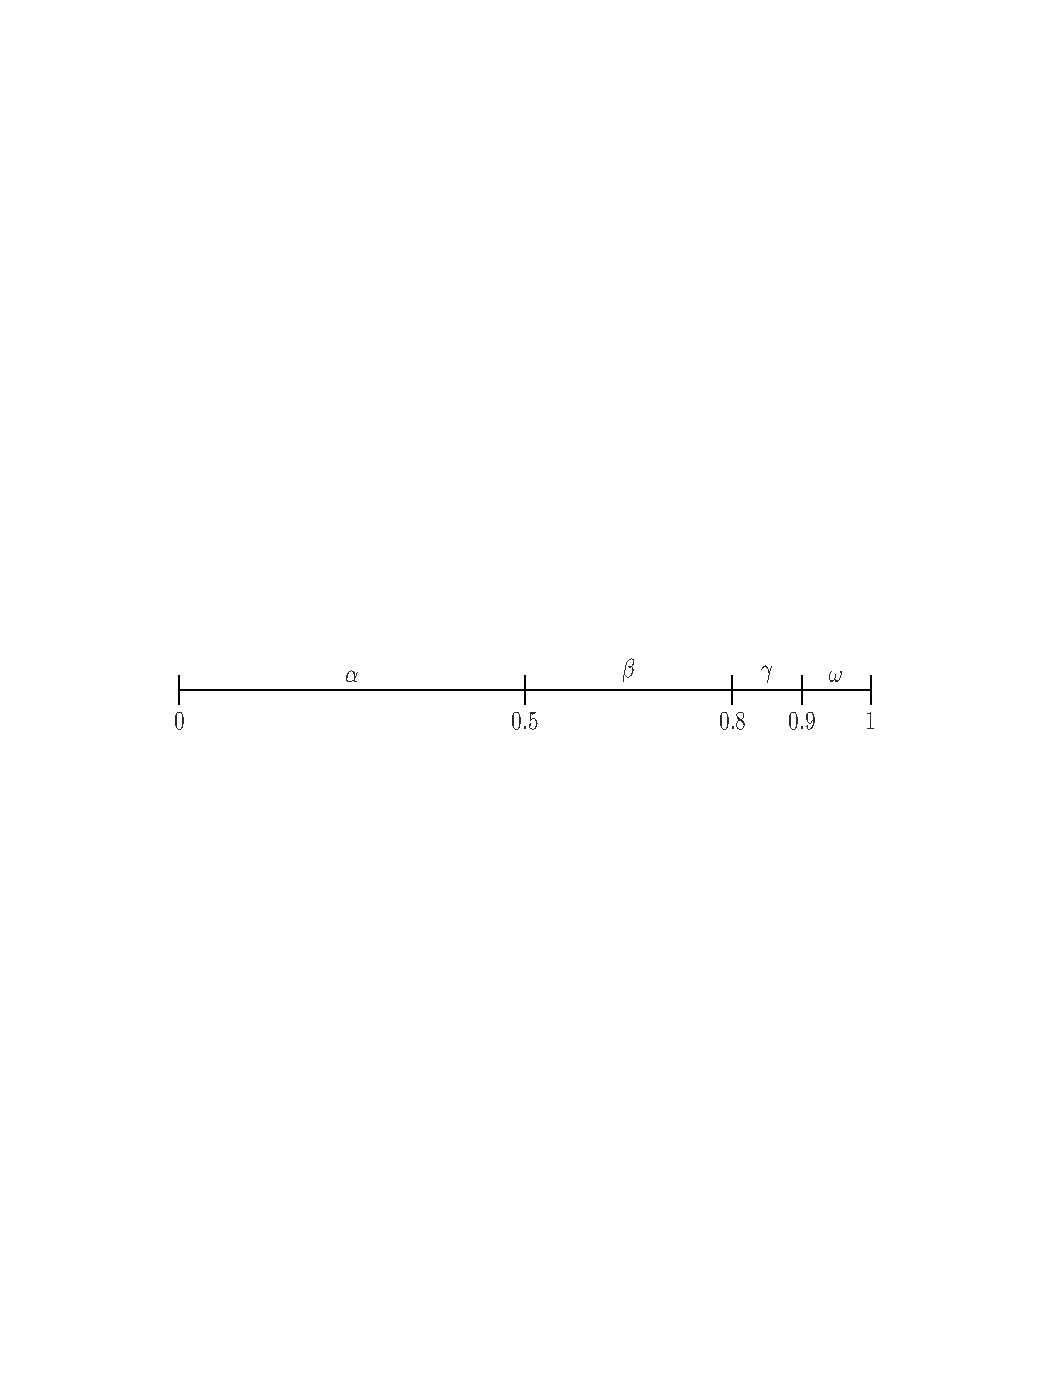
\includegraphics[scale=0.75]{Intervalo01} 
\end{center}
\caption{La partición de [0, 1) asociada con una distribución dada en $S^1$}
\label{fig:particion01}
\end{figure}

Generalmente, dada una cadena $X \in S^r$ denotamos por \textcolor{red}{$I_X$} el correspondiente intervalo:

\begin{center}
$I_X = [a(X), a(X) + P(X)). $
\end{center}

Para cada $r \geq 1$ estos intervalos forman una partición de [0, 1).

\end{frame} 
%%%%%%%%%%%%%%%%%%%%%%%%%%%%%%%%
\begin{frame}  \small 

\begin{definicion}[Código Aritmético]\label{CodeA}

\begin{itemize}
\item Supongamos que un código estacionario emite símbolos de un conjunto S y la probabilidad de distribución en $S^r$ es conocido.

\item Para $X \in S^r$ sea P = P(X), definimos $n_P$ el menor entero tal que $2^{n_P} \geq 1/P$, y sea $n = n_p +1$. 
\item La codificación aritmética $c: S^r \rightarrow B^{*}$ es definida tomando que c(X) sea la palabra $z_1z_2 \ldots z_n$ que representa el único entero c para el cual $c-1 \leq 2^n a(X) < c$.

\item Según el teorema \ref{th:Intervalo}, la condición $n = n_P + 1$ asegura que el número  $0.z_1z_2 \ldots z_n$ esta en el intervalo $I_X$ .

\end{itemize}


\end{definicion}


\end{frame} 
%%%%%%%%%%%%%%%%%%%%%%%%%%%%%%%%
\begin{frame}  \small 
\begin{ejemplo}

Sean $S = \{\alpha, \beta,\gamma ,\omega \}$. La siguiente tabla define una probabilidad de distribución en $S^2$: por ejemplo, el número en la fila $\beta$ y la columna $\gamma$  es la probabilidad de $\beta\gamma$

\begin{center}
 \begin{tabular}{ l c r r r}
         & $\alpha$ & $\beta$ & $\gamma$ & $\omega$\\
   $\alpha$    & 0.31 & 0.13 & 0.04 & 0.02 \\
   $\beta$      & 0.13 & 0.15 & 0.01 & 0.01\\
   $\gamma$ & 0.04 & 0.01 & 0.03 & 0.02\\
   $\omega$  & 0.02 & 0.01 & 0.02 & 0.05\\
 \end{tabular}
\end{center}

Determina el código aritmético para $S^2$.\\
\end{ejemplo}


\end{frame} 
%%%%%%%%%%%%%%%%%%%%%%%%%%%%%%%%
\begin{frame}  \small 

\textit{\underline{Solución}}:\\ 
\begin{itemize}
\item Para cada cadena $X \in S^2$ tomaremos \textcolor{red}{P} =P(X), \textcolor{red}{a} =a(X) y calcularemos 1/P, $\textcolor{red}{n_P}  \; | \; 2^{n_P} \geq 1/P$  y $\textcolor{red}{n}=n_P + 1$. 
\item Después determinaremos $c$ que cumpla que $c-1\leq 2^n a<c$, y establecemos c(X) la palabra binaria de longitud n correspondiente a c. 
\item Los cálculos para las primeros palabras codificadas son tabuladas a continuación. Notese que cada fracción $c/2^n$ está incluido en el intervalo [a, a + P ), como garantiza el teorema \ref{theorem:coding}.

\end{itemize}




\begin{center}
 \begin{tabular}{| l | l | l | l | l | l | l | l|}\hline
        		 \textbf{X}             & \textbf{P}      &   \textbf{a}    & \textbf{1/P} & \textbf{$n_P$ }&\textbf{ n} & \textbf{c }  & \textbf{c(X)}\\\hline\hline
   $\alpha\alpha$    & 0.31 & 0.00 & 3.2   & 2       & 3 & 1   & 001\\\hline
   $\alpha\beta$      & 0.13 & 0.31 & 7.7   & 3		 & 4 & 5   & 0101\\\hline
   $\alpha\gamma$ & 0.04 & 0.44 & 25    & 5		 & 6 & 29 & 011101\\\hline
   $\alpha\omega$  & 0.02 & 0.48 & 50    & 6      & 7 & 62 & 0111110\\\hline
   $\beta\alpha$     & 0.13 & 0.50 & 7.7    & 3      & 4 & 9   & 1001\\\hline
   $\ldots$              &  $\ldots$  &  $\ldots$  &  $\ldots$   &  $\ldots$ &  $\ldots$  &  $\ldots$  & $\ldots$ \\
 \end{tabular}
\end{center}



\end{frame} 
%%%%%%%%%%%%%%%%%%%%%%%%%%%%%%%%
\begin{frame}  \small 

Aunque hemos seguido un ejemplo \textcolor{red}{no es necesario calcular las palabras codificadas en orden}. 

\vspace{0.5cm}

Por ejemplo, si necesitamos la palabra codificada para $\gamma\beta$ podemos calcular directamente, conociendo solamente que $P(\gamma\beta) = 0.01$ y $a(\gamma\beta) = 0.84$.

\begin{center}
 \begin{tabular}{| l | l | l | l | l | l | l | l|}\hline
        		 X             & P       &   a    & 1/P & $n_P$  & n & c     & c(X)\\\hline\hline
   $\gamma\beta$    & 0.01 & 0.84 & 100   & 7       & 8 & 216  & 11011000\\\hline
   \end{tabular}
\end{center}


Si quisiera decodificar una palabra, por ejemplo 0111110, entonces:
\footnotesize
\begin{enumerate}
    \item Convierte $0.0111110_2$ a decimal: $0.0111110_2 = 1/4 + 1/8 + 1/16+ 1/32 + 1/64 =0.484375.$
    \item Busca el intervalo en la tabla donde esté  $0.484375$.
    $\alpha\omega: a=0.48, P = 0.02 \Rightarrow [a,a+P)=[0.48,0.50).$
    \item Comprueba pertenencia: $0.484375 \in [0.48,0.50)$.
\end{enumerate}

\footnotesize 
Nótese que no es una fuente sin memoria, ya que (por ejemplo)

P($\alpha$) = P ($\alpha\alpha$) + P ($\alpha\beta$) + P ($\alpha\gamma$) + P ($\alpha\omega$) = 0.31 + 0.13 + 0.04 + 0.02 = 0.5, y P($\alpha\alpha$) = 0.31 $\neq$ P ($\alpha$) $\times$ P ($\alpha$).

\end{frame} 



%%%%%%%%%%%%%%%%%%%%%%%%%%%%%%%%
%%%%%%%%%%%%%%%%%%%%%%%%%%%%%%%%
%EJERCICIOS %%%%%%%%%%%%%%%%%%%%%%%%%%%%%%%
%%%%%%%%%%%%%%%%%%%%%%%%%%%%%%%%
%%%%%%%%%%%%%%%%%%%%%%%%%%%%%%%%

%%%%%%%%%%%%%%%%%%%%%%%%%%%%%%%%
\begin{frame}  \small 

%4.16. Find the codeword for ωα in the arithmetic code for the distribution given in Example 4.18.

\begin{ejercicio}

Encuentra la palabra codificada  $\omega\alpha$ para el código aritmético en la distribución del anterior:
\end{ejercicio}

\pause
\textit{\underline{Solución}}:\\ 

\begin{center}
 \begin{tabular}{ l l l l l l l l}\hline
        		 X              & P       &   a     & 1/P & $n_P$  & n & c     & c(X)\\\hline\hline
   $\omega\alpha$    & 0.02 & 0.90	 & 50   & 6        & 7  & 116  & 1110100\\\hline
   \end{tabular}
\end{center}
\end{frame} 

%%%%%%%%%%%%%%%%%%%%%%%%%%%%%%%%
%%%%%%%%%%%%%%%%%%%%%%%%%%%%%%%%
\begin{frame}{Código en python}  \footnotesize

\begin{ejemplo}

Programas de ejemplo en python:

\begin{enumerate}
    \item syntheticCodev2.py: 
        \begin{itemize}
              \item  Generar textos sintéticos con alfabetos pequeños y control de entropía.
             \end{itemize}
            
    \item block arith codes.py:
    
            \begin{itemize}
              \item Construir el modelo de probabilidades de \alert{datagramas} .
              \item Codificar cada datagrama \(X\in S^r\) con una palabra binaria \(c(X)\).
              \item Medir tamaño comprimido, \emph{bits por carácter} (bpc) y \emph{ratio} comprimido/original.
            \end{itemize}
\end{enumerate}

\end{ejemplo}


\end{frame} 

%%%%%%%%%%%%%%%%%%%%%%%%%%%%%%%%
\begin{frame}[fragile] {Generador: \texttt{syntheticCodev2.py}}
\textbf{Uso:}
\begin{lstlisting}
# Maxima entropia (uniforme)
python3 syntheticCodev2.py --preset max -o uniform_20k.txt --show-stats

# Entropia media (por defecto 0.40,0.25,0.20,0.10,0.05)
python3 syntheticCodev2.py --preset mid -o mid_20k.txt --show-stats

# Minima entropia (muy sesgada)
python3 syntheticCodev2.py --preset min -o min_20k.txt --show-stats

# Probabilidades personalizadas
python3 syntheticCodev2.py --alphabet ABCDE \
  --probs 0.35,0.30,0.20,0.10,0.05 -n 30000 -o custom_30k.txt --show-stats
\end{lstlisting}


\end{frame}


%%%%%%%%%%%%%%%%%%%%%%%%%%%%%%%%
\begin{frame}[fragile] {Generador: \texttt{syntheticCodev2.py}}
\textbf{Ejemplo salida:}
\footnotesize
\begin{lstlisting}
python3 syntheticCodev2.py --preset max -o uniform_20k.txt --show-stats
 Generado uniform_20k.txt con 20000 simbolos.
- Configuracion -
Alfabeto: ABCDE
Probabilidades teoricas:
  A: 0.200000 (20.00%)
  B: 0.200000 (20.00%)
  C: 0.200000 (20.00%)
  D: 0.200000 (20.00%)
  E: 0.200000 (20.00%)
Entropia teorica H = 2.3219 bits/simbolo
Frecuencias observadas:
  A:   3911  ( 19.55%)
  B:   4025  ( 20.12%)
  C:   4092  ( 20.46%)
  D:   3999  ( 19.99%)
  E:   3973  ( 19.86%)
Entropia observada H_obs = 2.3218 bits/simbolo

\end{lstlisting}
\end{frame}

\begin{frame}[fragile]{Programa de codificación: \texttt{block\_arith\_codes.py}}
\textbf{Codificación:}
\begin{lstlisting}
python3 block_arith_codes.py encode mid_20k.txt --ngram 3 --show-table
\end{lstlisting}

\textbf{Salidas:}
\begin{itemize}
  \item \texttt{.barc}: flujo binario (concatenación de los \(c(X)\)).
  \item \texttt{.model.json}: tabla con \(X,P,a,1/P,n,c,c(X)\) y cola (tail).
  \item Métricas: tamaño original vs. comprimido, ratio, bpc, bits/token.
\end{itemize}

\textbf{Decodificación:}
\begin{lstlisting}
python3 block_arith_codes.py decode mid_20k.txt.ng3.barc \
  --model mid_20k.txt.ng3.barc.model.json -o decoded.txt
\end{lstlisting}
\end{frame}


% -----------------------------------------------------------
\begin{frame}{Ejemplo de tabla  generada}
\small
\begin{tabular}{lrrrrrrl}
\toprule
\(X\) & \(P\) & \(a\) & \(1/P\) & \(n_P\) & \(n\) & \(c\) & \(c(X)\) \\
\midrule
AA & 0.310000 & 0.000000 & 3.2 & 2 & 3 & 1  & 001 \\
AB & 0.130000 & 0.310000 & 7.7 & 3 & 4 & 5  & 0101 \\
AC & 0.040000 & 0.440000 & 25.0 & 5 & 6 & 29 & 011101 \\
AW & 0.020000 & 0.480000 & 50.0 & 6 & 7 & 62 & 0111110 \\
BA & 0.130000 & 0.500000 & 7.7 & 3 & 4 & 9  & 1001 \\
\bottomrule
\end{tabular}


\end{frame}
% -----------------------------------------------------------

\begin{frame}[fragile]{Demostración en vivo (sugerencias)}
\begin{lstlisting}
# 1) Generar datos
python3 syntheticCodev2.py --preset mid -o mid_20k.txt --show-stats

# 2) Codificar con distintos bloques
python3 block_arith_codes.py encode mid_20k.txt --ngram 1
python3 block_arith_codes.py encode mid_20k.txt --ngram 2
python3 block_arith_codes.py encode mid_20k.txt --ngram 3 --show-table --table-digits 8

# 3) Decodificar y verificar
python3 block_arith_codes.py decode mid_20k.txt.ng3.barc \
  --model mid_20k.txt.ng3.barc.model.json -o mid_20k_decoded.txt
\end{lstlisting}
\end{frame}

%4.17 Find the average word-length L2 for the code discussed in Example 4.18. [You do not need to calculate the codewords.] Compare the values of L2/2, H(p1), and H(p2)/2.
%4.18 Construct the arithmetic code for the probability distribution on S2 given in Example 4.7, taking a < b < c. Compare the result with the Huffman code for this source.
%4.19 A memoryless source is defined by the distribution P on S, which determines the distributions (also denoted by P) on Sr for all r ≥ 2. Show that the corresponding cumulative distribution functions sat- isfy the equation a(x1x2 ...xr) = a(x1x2 ...xr−1)+P(x1x2 ...xr−1)a(xr).
%4.20 Deduce from the previous exercise that, in the memoryless case, the value of a(X) for a string X ∈ Sr can be computed given only the values of P(s) and a(s) for the symbols s that occur X. Illus- trate your answer by writing down a set of equations for calculating a(βωγβ) when S contains the symbols α < β < γ < ··· < ω.
%%%%%%%%%%%%%%%%%%%%%%%%%%%%%%%%
\begin{frame}  \footnotesize
\begin{ejercicio}
Establezca la longitud media $L_2$ para el código anterior. (No es necesario calcular las palabras codificadas). Compara los valores de $L_2/2$, $H(p^1)$, $H(p^2)/2$
\end{ejercicio}
\end{frame} 
%%%%%%%%%%%%%%%%%%%%%%%%%%%%%%%%

%%%%%%%%%%%%%%%%%%%%%%%%%%%%%%%%
\begin{frame}  \tiny
\textit{\underline{Solución}}:\\ 
\begin{center}
 \begin{tabular}{ c c c c c c c c}
        		 X             & P      &   a    & 1/P & $n_P$ \\\hline\hline
   $\alpha\alpha$    & 0.31 & 0.00 & 3.2   & 2       \\\hline
   $\alpha\beta$      & 0.13 & 0.31 & 7.7   & 3		 \\\hline
   $\alpha\gamma$ & 0.04 & 0.44 & 25    & 5		 \\\hline
   $\alpha\omega$  & 0.02 & 0.48 & 50    & 6      \\\hline
  
   $\beta\alpha$      & 0.13 & 0.50 & 7.7    & 3      \\\hline
   $\beta\beta$        & 0.15 & 0.63 &  6.6   &   3    \\\hline
   $\beta\gamma$   & 0.01 & 0.78  &  100   &   7    \\\hline
   $\beta\omega$    & 0.01 & 0.79 &   100  &    7   \\\hline
   
   $\gamma\alpha$    & 0.04 & 0.80 &  25   &    5   \\\hline
   $\gamma\beta$      & 0.01 & 0.84 &  100  &   7    \\\hline
   $\gamma\gamma$ &  0.03&  0.85&   33,33  & 6      \\\hline
   $\gamma\omega$  &  0.02& 0.88 &    50 &   6    \\\hline

   $\omega\alpha$      & 0.02 & 0.90&   50 &     6  \\\hline
   $\omega\beta$        & 0.01& 0.92 & 100  &    7   \\\hline
   $\omega\gamma$   & 0.02& 0.93 &    50 &    6   \\\hline
   $\omega\omega$    & 0.05& 0.95 &    20 &     5  \\\hline
 \end{tabular}
\end{center}

\footnotesize
$L_2 = 1 + \sum p_i \times n_p $ = 2 * 0,31 + 3 *0,13+ 5 *0,04 + 6 *0,02 + 3 *0,13 + 3*0,15 + 7 * 0,01 + 7 *0,01 + 5 *0,04 + 7 * 0,01 +6 *0,03 + 6 * 0,02 +6* 0,02 + 7* 0,01 + 6 * 0,02 + 5 *0,05= 1+ 3,44 = 4,44.\\

\vspace{0.5cm}

$L_2/2$= 2.22. \\
$H(p^1)$ = 1.685.\\
$H(p^2)/2$ = 1.495. 

\end{frame} 
%%%%%%%%%%%%%%%%%%%%%%%%%%%%%%%%
%%%%%%%%%%%%%%%%%%%%%%%%%%%%%%%%
\begin{frame}  \footnotesize

\begin{ejercicio}
Construya el código aritmético para la distribución de probabilidad en $S^2$ dado en el ejemplo \ref{ej:4.7}, tomando $a< b < c$.
Compare los valores de $L_2/2$, $H(p^1)$, $H(p^2)/2$. [No es necesario establecer las palabras codificadas]

\begin{center}
 \begin{tabular}{ l c r r}
         & a & b & c\\
   a & 0.39 & 0.17 & 0.04 \\
   b & 0.15 & 0.11 & 0.04 \\
   c & 0.06 & 0.02 & 0.02 \\
 \end{tabular}
\end{center}

\end{ejercicio}
\end{frame} 

\begin{frame}  \footnotesize

\textit{\underline{Solución}}:\\ 

\begin{center}
 \begin{tabular}{ c c c c c c c c}
    X     &  P     &   a    & 1/P & $n_P$ & n & c   & c(X)\\\hline\hline
   aa    & 0.39 & 0.00 & 2.5    & 2      & 3 & 1    & 001\\\hline
   ab    & 0.17 & 0.39 & 5.8    & 3		& 4 & 7    & 0111\\\hline
   ac    & 0.04 & 0.56 & 25     & 5		& 6 & 36  & 100100 \\\hline
   ba    & 0.15 & 0.60 & 6.6    & 3      & 4 & 10  & 1010\\\hline
   bb    & 0.11 & 0.75 & 9.1    & 4      & 5 & 25  & 11001\\\hline
   bc    & 0.04 & 0.86 & 25     & 5      & 6 & 56  & 111000 \\\hline
   ca    & 0.06 & 0.90 & 16.6  & 5      & 6 & 58    & 111010\\\hline
   cb    & 0.02 & 0.96 & 50     & 6      & 7 & 123  & 1111011\\\hline
   cc    & 0.02 & 0.98 & 50     & 6      & 7 & 126  & 1111110 \\\hline
   
 \end{tabular}
\end{center}

\vspace{0.5cm}
$L_2= \sum p_i * n = 1+ \sum p_i * n_p =$ 3 * 0,39 + 4 *0,17 + 6*0,04 + 4 *0,15 + 5* 0,11 + 6* 0,04+ 6 * 0,06 + 7 * 0,02 + 7 *0,02 =4,12. \\

$L_2/2$=2.06\\

$H(p^1)= 1,295$. \\
$H(p^2)= 2,566$;  \\
$H(p^2)/2 = 1,283$\\

\end{frame} 



%%%%%%%%%%%%%%%%%%%%%%%%%%%%%%%%
\begin{frame}  \footnotesize

\begin{itemize}
\item Hemos mostrado en la codificación aritmética que pueden ser construidos de forma aislada, por lo que en la práctica es más eficiente que utilizar la regla de Huffman. 

\item Nos queda establecer que la codificación aritmética tiene las propiedades deseables: 

\begin{itemize}
\item  (i) el código es libre de prefijo, por lo que la codificación puede ser realizada `en linea', y 
\item (ii) el código es cercano al óptimo. Estos hechos son consecuencia de la elección $n = n_P  +1 $ en la definición y  garantizar que \(c/2^n \in [a,a+P)\).
\end{itemize}
\end{itemize}



\begin{teorema}
Un código aritmético construida acorde la definición \ref{CodeA} es libre de prefijo.
\end{teorema}


\begin{teorema}
Sea P una probabilidad en el conjunto $S^r$ de cadenas de longitud r, y sea L la longitud media de palabra del correspondiente código aritmético. Entonces

\begin{center}
$L < H(P) + 2.$
\end{center}
\end{teorema}

%+1	Efecto del redondeo a longitud entera de bits
%+1 adicional	Margen para asegurar que la fracción c /2^n cae dentro del intervalo [a,a+P))

\end{frame} 
%%%%%%%%%%%%%%%%%%%%%%%%%%%%%%%%%%%%%%%%%%%%%%%%%%%%%%%%%%%%%%%%%%%%%%%%%%%%%%%%%%%%%%%%%%%%%%%%
%%%%%%%%%%%%%%%%%%%%%%%%%%%%%%%%%%%%%%%%%%%%%%%%%%%%%%%%%%%%%%%%
%%%%%%%%%%%%%%%%%%%%%%%%%%%%%%%%%%%%%%%%%%%%%%%%%%%%%%%%%%%%%%%%
%%%%%%%%%%%%%%%%%%%%%%%%%%%%%%%%
\subsection{Codificación con un diccionario dinámico}

%%%%%%%%%%%%%%%%%%%%%%%%%%%%%%%%
\begin{frame}   \footnotesize
{
\setbeamercolor{block title}{bg=blue!40!black, fg=white}
\setbeamercolor{block body}{bg=white!05, fg=black}
\begin{block}{Sección 4.2}
Codificación con un diccionario dinámico
\end{block}
}
\end{frame} 
%%%%%%%%%%%%%%%%%%%%%%%%%%%%%%%%
%%%%%%%%%%%%%%%%%%%%%%%%%%%%%%%%
\begin{frame} \frametitle{Codificación con un diccionario dinámico} \footnotesize 

\begin{definicion} [Diccionario, indice]
Un diccionario D basado en el alfabeto S es una secuencia de palabras distintas en $S^*$:
\begin{center}
$D = d_1,d_2,d_3, \ldots ,d_N$
\end{center}
Además establecemos que el indice de $d_i$ es i.
\end{definicion}

\begin{itemize}
\item En la codificación aritmética impusimos un ``orden alfabetico'' en el conjunto de símbolos S, y construimos el correspondiente ``orden diccionario'' en $S^r$. 


\item  Por ejemplo, si S tiene tres símbolos en el orden $\alpha < \beta < \gamma$, el conjunto $S^2$ es un diccionario con el orden 

	\begin{center}
$\alpha\alpha , \alpha\beta, \alpha\gamma , \beta\alpha, \beta\beta, \beta\gamma, \gamma\alpha, \gamma\beta, \gamma\gamma$
\end{center}

\item  y el indice del elemento $\gamma\alpha$ es 7.  

\item Este es un ejemplo de diccionario estático. 
\end{itemize}

\end{frame} 
%%%%%%%%%%%%%%%%%%%%%%%%%%%%%%%%
\begin{frame}  \small 

\begin{itemize}
\item  En esta sección consideramos un método de codificación en el cual el diccionario es dinámico, en otras palabras es construido durante el proceso, por lo que contiene aquellas cadenas que ocurren en un mensaje dado. 

\item Asumimos que la fuente es estacionaria por lo que las cadenas de símbolos que suceden en el comienzo del mensaje son las típicas que ocurrirán mas adelante, por lo que no necesitamos información especifica sobre la distribución de los símbolos.

\item Describimos el sistema de codificación Lempel-Ziv-Welch, también conocido como LZW.


\end{itemize}


\end{frame} 
%%%%%%%%%%%%%%%%%%%%%%%%%%%%%%%%
\begin{frame}  \small 

\begin{itemize}

\item  El alfabeto S tiene el tamaño m, con símbolos $s_1 < s_2 < \ldots < s_m$. Tanto codificador como decodificador comienzan con el diccionario 

\begin{center}
$D_0 = d_1,d_2, \ldots ,d_m,$	donde $d_i = s_i$ (i = 1,2,$\ldots$,m).
\end{center}

\item Si el mensaje es $X= x_1 x_2 \ldots x_n$, donde $x_i \in S$ (i = 1,2,$\ldots$,m), 

\item El codificador hace una codificación del mensaje, c(X) y al mismo tiempo construye un diccionario $D_X$ añadiendo a $D_0$ ciertas cadenas $s_p s_q \ldots$ que ocurre en X. 

\item La regla de codificación reemplaza cada cadena por su índice en $D_X$. 

\item El decodificador utiliza la secuencia de números c(X), y el diccionario inicial $D_0$, para reconstruir X y $D_X$.
\end{itemize}
\end{frame} 


%%%%%%%%%%%%%%%%%%%%%%%%%%%%%%%%
\begin{frame}  \small 

\begin{definicion} [Codificación LZW] \label{def:LZW}

Supongase que un mensaje $X = x_1 x_2 \ldots x_n$ en el alfabeto $S=\{s_1, s_2, \ldots, s_m\}$ dado. Sea $D_0= d_1, d_2, \ldots, d_m$, donde $d_i =s_i$  $(i = 1,2,\ldots,m)$. 

La reglas de codificación LZW construye $c(X ) = c_1 c_2 c_3 \ldots$ en una serie de pasos.

\begin{itemize}

\item  Paso 1.	El primer símbolo $x_1$ (= $s_p$ ) es una entrada $d_p$ en $D_0$. 

\begin{enumerate}
\item Codificamos $x_1$ definiendo $c_1 = p.$

\item La cadena $x_1x_2 (= s_p s_q )$ no esta en $D_0$. Definimos

\begin{center}
$d_{m+1} = x_1x_2$,	$D_1 = (D_0, d_{m+1})$.
\end{center}

\end{enumerate}


\item Continua...
\end{itemize}

\end{definicion}

\end{frame} 


%%%%%%%%%%%%%%%%%%%%%%%%%%%%%%%%
\begin{frame}  \small 

\begin{definicion} [Codificación LZW (Continuación] 

\begin{itemize}

\item Paso k $(k \geq 2)$ Supongase que hemos completado los pasos 1, 2, $\ldots$, k-1. Esto significa que el código $c_1 c_2 \ldots c_{k-1}$ para un segmento inicial $x_1 x_2 \ldots x_i$ de X, y además hemos construido un diccionario $D_{k-1}= d_1, d_2, \ldots, d_{m+k-1}$.Encontrar la cadena más larga w de la forma

\begin{center}
$w = x_{i+1} \ldots x_j	(j \geq i + 1)$
\end{center}

tal que w está en $D_{k-1}$, sea $w=d_t$. Tal cadena existe, debido a que $x_{i+1}$ es un solo símbolo y ya está incluido en el diccionario inicial $D_0$. Por definición, $wx_{j+1}$ no esta en $D_{k-1}$.  Codificamos el segmento $x_{i+1}\ldots x_j$ de X mediante 

\begin{center}
$c_k = t$,	y define $d_{m+k} = wx_{j+1}$,	$D_k = (D_{k-1}, d_{m+k})$.
\end{center}

\item Repetir el procedimiento hasta alcanza el final del mensaje.

\end{itemize}

\end{definicion}

\begin{teorema}
Un código LZW construido siguiendo la Definición \ref{def:LZW} es unívocamente decodificable.
\end{teorema}


\end{frame} 


%%%%%%%%%%%%%%%%%%%%%%%%%%%%%%%%
\begin{frame}  \small 

\begin{ejemplo}

Siendo el alfabeto S = \{A, B, C, D, R\} y aplicar las reglas de codificación LZW al mensaje

\begin{center}
X = ABRACADABRA
\end{center}	

\end{ejemplo}
\pause
\textit{\underline{Solución}}:\\

Comenzamos con el diccionario $D_0 = A, B, C, D, R$. La regla para el Paso 1, nos indica que codifiquemos A, el cual tiene indice 1 y añadimos $AB$ al diccionario:

\begin{center}
c(A) = 1,	$D_1$ = A,B,C,D,R,AB.
\end{center}

En el paso 2, $B$ está en $D_1$ pero no $BR$, por lo que codificamos $B$ por su indice 2 y añadimos $BR$:

\begin{center}
c(AB) = 1 2,	$D_2$ = A,B,C,D,R,AB,BR.
\end{center}


\end{frame} 
%%%%%%%%%%%%%%%%%%%%%%%%%%%%%%%%

%%%%%%%%%%%%%%%%%%%%%%%%%%%%%%%%
\begin{frame}  \small 

Las reglas dicen que en los Pasos 3,4,5,6,7 continuamos de una forma similar hasta que alcanzamos el estado:

\begin{center}
c(ABRACAD) = 1 2 5 1 3 1 4,\\	$D_7$ = A,B,C,D,R,AB,BR,RA,AC,CA,AD,DA.
\end{center}

En el Paso 8 $AB$ ya está en $D_7$, con índice 6, pero $ABR$ no está en $D_7$, por lo que el estado es 

\begin{center}
c(ABRACADAB) = 1 2 5 1 3 1 4 6, \\
$D_8$ = A,B,C,D,R,AB,BR,RA,AC,CA,AD,DA,ABR.
\end{center}

En el Paso 9, $RA$ está en el diccionario, con indice 8, y el mensaje finaliza, por lo que 

\begin{center}
c(ABRACADABRA) = 1 2 5 1 3 1 4 6 8.
\end{center}


\end{frame} 


%%%%%%%%%%%%%%%%%%%%%%%%%%%%%%%%
\begin{frame}  \small 

\begin{ejemplo}
Dado el diccionario $D_0$= I,M,P,S, decodifica el mensaje

\begin{center}
214468331
\end{center} 
\end{ejemplo}
\pause
\textit{\underline{Solución}}:\\

En el Paso 1, $c_1 =2$ y $d_2 = M$ por lo que $x_1=M$. También $c_2=1$ y $d_1=I$ por lo que la nueva entrada en el diccionario es $MI$.

\begin{center}
$2 \mapsto M$ ,	$D_1 = I , M , P , S , MI $
\end{center}

En el Paso 2, $c_2=1$ y $d_1=I$ por lo que $x_2=I$. Además $c_3 = 4$ y $d_4=S$, por tanto la nueva entrada en el diccionario es $IS$. Por tanto,

\begin{center}
$2 1\mapsto MI$ ,	$D_1 = I , M , P , S , MI, IS $
\end{center}
\end{frame} 
	
%%%%%%%%%%%%%%%%%%%%%%%%%%%%%%%%
\begin{frame}  \small 	
Los Pasos 3 y 4 son similares, y tienen como resultado 

\begin{center}
$2 1 4 4\mapsto MISS$ ,	$D_4 = I , M , P , S , MI, IS, SS, SI $
\end{center}

En el siguiente paso $c_5=6,$ y $d_6=IS$ por lo que $x_5=I, x_6=S.$ También $c_6=8$ y $d_8=SI$ por tanto la entrada del diccionario es $ISS$.
Por tanto,

\begin{center}
$2 1 4 4 6\mapsto MISSIS$ ,	$D_5 = I , M , P , S , MI, IS, SS, SI, ISS $
\end{center}

Pasos 7,8,9 son similares, y el resultado es  

\begin{center}
$2 1 4 4 6 8 3 3 1 \mapsto MISSISSIPPI$
\end{center}


\end{frame} 


%%%%%%%%%%%%%%%%%%%%%%%%%%%%%%%%
\begin{frame}  \small 

\begin{itemize}
\item En este punto, podemos plantearnos porqué las reglas LZW alcanzan una compresión importante.  

\item En estos ejemplos, solo alcanzamos una pequeña cantidad de compresión con el costo asociado.

\item Por ejemplo, el mensaje $ABRACADABRA$ tiene longitud 11, y la codificación $1 2 5 1 3 1 4 6 8$ tiene una longitud de 9. 

\item Sin embargo en la práctica cuando el mensaje incrementa en longitud, con el inevitable incremento de cadenas, entonces se produce una mejora.

\item En la práctica, LZW ofrece unos buenos resultados.

\end{itemize}
 

\end{frame} 

%%%%%%%%%%%%%%%%%%%%%%%%%%%%%%%%
%%%%%%%%%%%%%%%%%%%%%%%%%%%%%%%%
\begin{frame}{Código en python}  \footnotesize

\begin{ejemplo}

Programa de ejemplo en python:

\begin{enumerate}\footnotesize
    \item lzw.py: \footnotesize
        \begin{itemize}\footnotesize
            \item Construir el \alert{diccionario inicial} con los símbolos únicos del texto (alfabeto).
            \item Recorrer el texto añadiendo nuevas entradas \(w+k\) al diccionario cada vez que no existan.
            \item Emitir el código correspondiente a cada cadena \(w\) encontrada en el diccionario.
            \item Generar el fichero comprimido con cabecera (\texttt{LZW1}), alfabeto inicial y secuencia de códigos.
        \end{itemize}
\end{enumerate}

\end{ejemplo}


\end{frame} 

%%%%%%%%%%%%%%%%%%%%%%%%%%%%%%%%
\begin{frame}[fragile] {Generador: \texttt{lzw.py}}
\textbf{Uso:}
\begin{lstlisting}
# Codificar con tabla de pasos
python3 lzw.py encode uniform_20k.txt --show-steps --colw 30 -o uniform_20k.lzw --output-json uniform_20k.meta.json

# Inspeccionar el binario
python3 lzw.py inspect uniform_20k.lzw

# Decodificar
python3 lzw.py decode uniform_20k.lzw -o uniform_20k.out.txt
\end{lstlisting}


\end{frame}


%%%%%%%%%%%%%%%%%%%%%%%%%%%%%%%%
\begin{frame}[fragile] {Generador: \texttt{lzw.py}}
\footnotesize
\begin{verbatim}

   i | w         |   k   |   emit | add to dict                   
------------------------------------------------
   1 | E         |   E   |        |                               
   2 | E         |   C   |      0 | EC                            
   3 | C         |   A   |      1 | CA                            
   4 | A         |   E   |      2 | AE                            
   5 | E         |   E   |      0 | EE                            
   6 | EC        |   C   |        |                               
   7 | EC        |   D   |      5 | ECD                           
   8 | D         |   A   |      3 | DA                            
   9 | A         |   D   |      2 | AD                            
  10 | D         |   B   |      3 | DB            

\end{verbatim}
\footnotesize
\textbf{i}	$-->$ Número de paso (iteración del algoritmo)\\
\textbf{w}	$-->$ Cadena actual (la más larga encontrada en el diccionario hasta ahora)\\
\textbf{k}	$-->$ Siguiente símbolo leído del texto\\
\textbf{emit} $-->$	Código numérico emitido al flujo de salida\\
\textbf{add to dict}	 $-->$ Nueva entrada añadida al diccionario (concatenación w+k)\\

\end{frame}


           %%%%%%%%%%%%%%%%%%%%%%%%%%%%%%%%
\begin{frame}[fragile] {Output: \texttt{uniform\_20k.lzw}}
\footnotesize
\begin{verbatim}
4c5a 5731 0500 0000 0100 0000 4501 0000
0043 0100 0000 4101 0000 0044 0100 0000
429e 1200 0000 0000 0000 0000 0001 0000
0002 0000 0000 0000 0005 0000 0003 0000
0002 0000 0003 0000 0004 0000 000b 0000
\end{verbatim}
\footnotesize
4c 5a 57 31	$\rightarrow$ ASCII ``LZW1''\\
05 00 00 00	$\rightarrow$  m = 5 símbolos en el alfabeto\\
0100 0000 45 $\rightarrow$ len=1, símbolo `E'\\
0100 0000 43 $\rightarrow$ len=1, símbolo `C'\\
0100 0000 41 $\rightarrow$ len=1, símbolo `A'\\
0100 0000 44 $\rightarrow$ len=1, símbolo `D'\\
0100 0000 42 $\rightarrow$ len=1, símbolo `B'\\
9e 1200 0000 0000 0000 0000 $\rightarrow$ 4766 códigos\\
0001 0000 $\rightarrow$ símbolo 1\\
0002 0000 $\rightarrow$ símbolo 2\\
0000 0000 $\rightarrow$ símbolo 0\\
0005 0000 $\rightarrow$ símbolo 5\\
0003 0000 $\rightarrow$ símbolo 3\\

\end{frame}     


%%%%%%%%%%%%%%%%%%%%%%%%%%%%%%%%
%%%%%%%%%%%%%%%%%%%%%%%%%%%%%%%%
%%%%%%%%%%%%%%%%%%%%%%%%%%%%%%%%
%SECCION %%%%%%%%%%%%%%%%%%%%%%%%%%%%%%%
%%%%%%%%%%%%%%%%%%%%%%%%%%%%%%%%
%%%%%%%%%%%%%%%%%%%%%% 

%%%%%%%%%%%%%%%%%%%%%%%%%%%%%%%%
%%%%%%%%%%%%%%%%%%%%%%%%%%%%%%%%
%\begin{frame}  \small \begin{ejercicio} \end{ejercicio} \pause \textit{\underline{Solución}}:\\ \end{frame} 
%%%%%%%%%%%%%%%%%%%%%%%%%%%%%%%%
%%%%%%%%%%%%%%%%%%%%%%%%%%%%%%%%
%EJERCICIO %%%%%%%%%%%%%%%%%%%%%%%%%%%%%%%
%%%%%%%%%%%%%%%%%%%%%%%%%%%%%%%%

%%%%%%%%%%%%%%%%%%%%%%%%%%%%%%%%
%\begin{frame}  \small  
%\begin{itemize} \item  \item \item \item 
%\end{itemize} \end{frame} 

%%%%%%%%%%%%%%%%%%%%%%%%%%%%%%%%
%\begin{frame}  \small  
%\end{frame} 





\begin{frame} %\frametitle{Preguntas}

%\begin{center}
%¡Gracias por su atención!\\
%\end{center}
\vspace*{2cm}

\begin{center}
\textbf{José A. Montenegro Montes} \\

\textit{Dpto. Lenguajes y Ciencias de la Computación}\\
\textit{ETSI  Informática. Universidad de Málaga}\\
\textbf{jmmontes@uma.es}\\
%\href{https://twitter.com//monteDocencia}{
%
\includegraphics[height=0.05\textheight]{twitter.jpg}}
\end{center}

\vspace*{1,5cm}


\includegraphics[height=0.15\textheight]{logoUma.jpg} \hspace*{3.6cm}

\includegraphics[height=0.15\textheight]{logoInf.jpg}   \hspace*{3.7cm}

\includegraphics[height=0.15\textheight]{logoLcc.jpg}  




\end{frame} 

\end{document} 